\documentclass {article}

\usepackage[letterpaper]{geometry}
\usepackage{amsthm, amsmath, amssymb, stmaryrd}
\usepackage{graphicx, hyperref}
\usepackage{plstx, listproc}
 
\newtheorem{theorem}{Theorem}[section]
\newtheorem{lemma}[theorem]{Lemma}


\title {Verifier Design}
\author {Jenna Wise, Cameron Wong, Jonathan Aldrich, Johannes Bader, \'{E}ric Tanter}
\date {\today}

%% Commands
\newcommand{\lcar}{\left<}
\newcommand{\rcar}{\right>}
\newcommand{\true}{\text{true}}
\newcommand{\eif}[3]{if \ ( #1 ) \ \{ #2 \} \ else \ \{#3\}}
\newcommand{\fphi}{\widehat{\phi}}
\newcommand{\tphi}{\widetilde{\phi}}
\newcommand{\acc}[1]{\text{acc}(#1)}
\newcommand{\imp}{\Rightarrow}
\newcommand{\timp}{\ \widetilde{\Rightarrow}\ }
\newcommand{\maximp}[2]{\underset{\Rightarrow}{\text{max}}\left\{#1 \mid #2\right\}}

\newcommand{\wlp}[2]{\text{WLP}(#1,#2)}
\newcommand{\twlp}[2]{\widetilde{\text{WLP}}(#1,#2)}
\newcommand{\swlp}[2]{\text{sWLP}(#1,#2)}
\newcommand{\swlpi}[2]{\text{sWLP}_i(#1,#2)}

% uppercase word defs
\newcommand{\satdef}{\textsc{SatFormula}}

\begin{document}

\maketitle

\section{Verification Design}
[OVERALL VERIFICATION DESIGN - TBD]

%[TALK ABOUT OVERALL DESIGN HERE]
%[REFER TO SUBSECTIONS FOR MORE DETAIL ON OVERALL DESIGN PIECES]
%Gradual verifier supports implicit dynamic frames for reasoning about the heap and gradual verification for ...
%
%Explain what protocol buffers are
%
%Explain intention to implement Java, Wyvern, and C0 frontends [C0 may be a special case if it is written in Ocaml].
%
%Explain that we can perform dynamic checks in the verifier and translate the results in the language specific frontend, but either way the translation must take place and in which case we decide to employ the existing runtime mechanisms of the target language; this is important for c0 which already performs other runtime checks or has mechanisms to do so?
%
\begin{figure}[!ht]
	\centering
	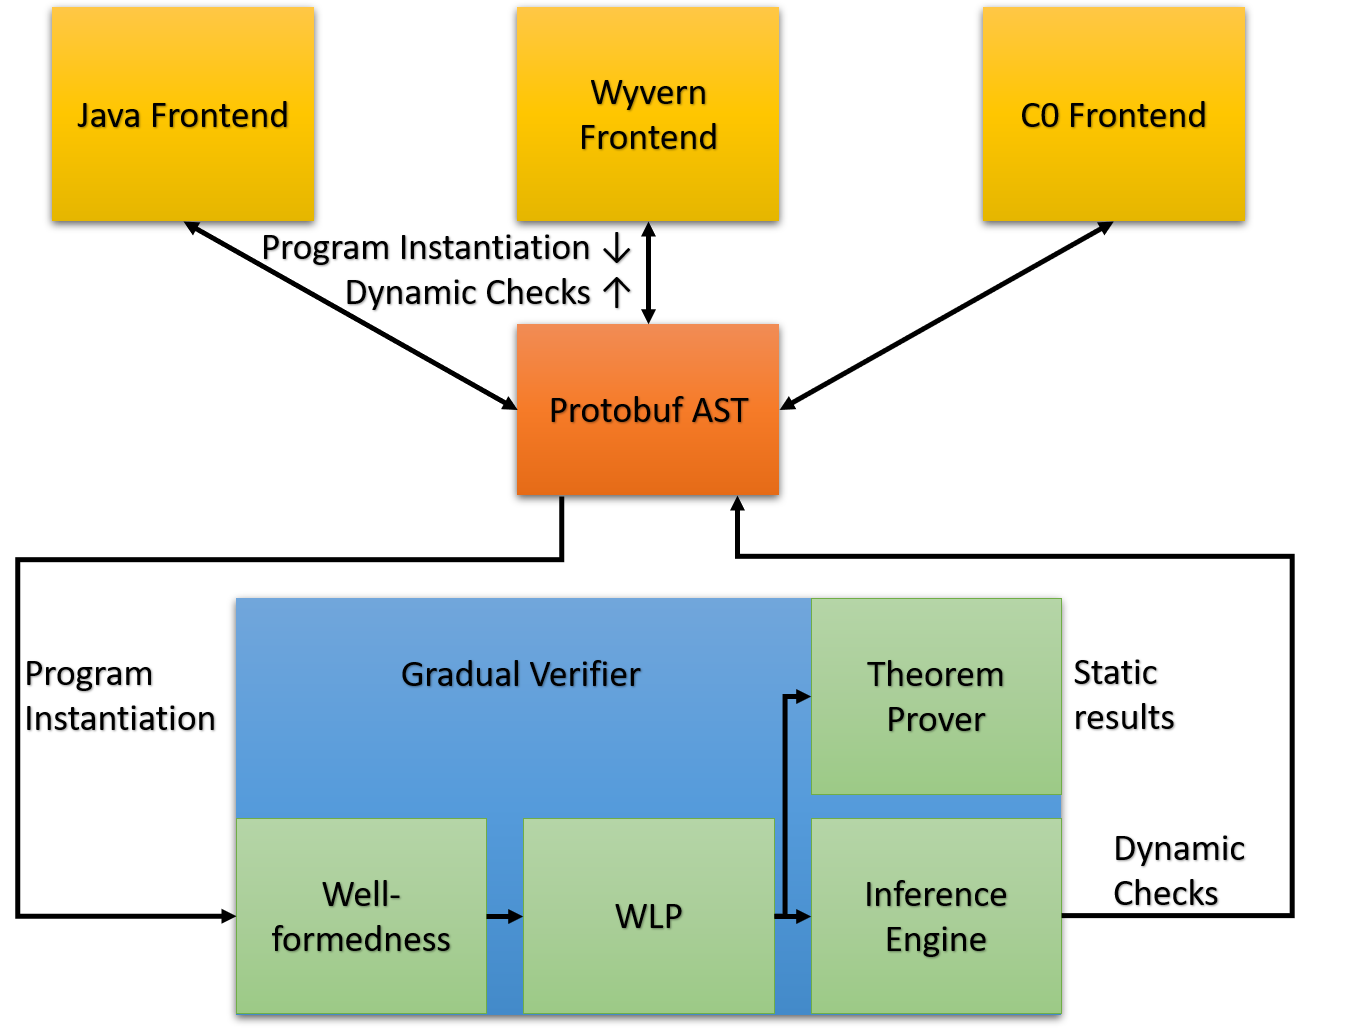
\includegraphics[width=15cm]{resources/architecture}
	\caption{TBD - Not final version of diagram, changes coming, particularly to the WLP, Inference Engine, and Theorem Prover part of the diagram}
	\label{fig:architecture}
\end{figure}

\subsection{Language Dependent Frontend}
The gradual verifier supports multiple programming languages through protocol buffers [CITE protobuf] and language dependent frontends. Language dependent frontends must do the following:

\begin{itemize}
\item Check well-formedness of the program to be verified
	\begin{itemize}
	\item This includes type-checking the program
	\end{itemize}
\item Use generated code from the protocol buffer message types of the gradual verifier's core language AST .proto file to
	\begin{itemize}
	\item Translate the program to be verified into a program written in the gradual verifier's core language
	\item Receive and execute dynamic checks determined necessary by the gradual verifier
	\end{itemize}
\end{itemize}

Since the language dependent frontends must translate the program to be verified into a program written in the gradual verifier's core language, the programs and language features that can be verfied are restricted to the programs and language features that are supported by the verifier and its core language.

Frontends are available for the Java, Wyvern, and C0 programming languages which can be found at [LINK(S) HERE].

[DISCUSS ONE OF THEM HERE? - TBD]

%A special case of this process occurs when a programming languages's compiler is written in Ocaml as is the case with the C0 language. .... [mention Ocaml verifier, which won't require use of protobuf as much]
\subsection{Gradual Verifier}
[SUMMARY OF GRADUAL VERIFIER TBD]
% The gradual verifier supports a smooth continuum between static and dynamic verification by implementing the idea of gradual verification presented by Bader et al. [CITE]. It does this by allowing users to write imprecise specifications that are verified
% implemented in Ocaml
% modular verification, IDF for reasoning about heap dependent structures
% talk about each subsubsection

\subsubsection{Core language}
The gradual verifier is dependent on a core language seen in BNF grammar format in Figure \ref{fig:core-grammar}. A language independent version of the core language grammar is available as protocol buffer message types in our Github repository (\href{https://github.com/wyvernlang/grad-ver/blob/master/src/ast/ast.proto}{here}). 

Note that there are discrepancies between the core language grammar as seen in Figure \ref{fig:core-grammar} and its language independent counterpart, because we anticipate implementing additional language features for verification in the near future. The core language BNF grammar shows language features that can be verified currently, while the language independent counterpart shows language features that can be verified currently and additional features that will be verifiable in the future.


\begin{figure}[ht!]
\begin{plstx}
*(variables): x,y,z [\in] \mathit{VAR} \\
*(values): v [\in] \mathit{VAL} \\
*(expressions): e [\in] \mathit{EXPR} \\
*(statements): s [\in] \mathit{STMT} \\
*(object Ids): o [\in] \mathit{LOC} \\
*(field names): f [\in] \mathit{FIELDNAME} \\
*(method names): m [\in] \mathit{METHODNAME} \\
*(class names): C, D [\in] \mathit{CLASSNAME} \\
: P ::= \overline{cls} \ s \\
: cls ::= class \ C \ extends \ D \ \{\overline{\mathit{field}} \ \overline{method}\} \\
: \mathit{field} ::= T \ f; \\
: T ::= int | C | \top \\
: method ::= T \ m(\overline{T \ x}) \ contract \ \{s\} \\
: contract ::= requires \ \tphi \ ensures \ \tphi \\
: \oplus ::= + | - | \ast | \backslash \\
: \odot ::= \neq | = | < | > | \leq | \geq \\
: s ::= skip | s_1 \ ; \ s_2 | T \ x := e | \eif{x \odot y}{s_1}{s_2} | x.f := y | x := new \ C | y := z.m(\overline{x}) | assert \ \phi | release \ \phi | hold \ \phi \ \{ s \} \\
: e ::= v | x | e \oplus e | e.f \\
: x ::= result | id | old(id) | this \\
: v ::= n | o | null \\
: \phi ::= \true | e \odot e | acc(e.f) | \phi \ast \phi \\
: \tphi ::= \phi | ? \ast \phi \\
\end{plstx}
\caption{The gradual verifier's core language in BNF grammar format}
\label{fig:core-grammar}
\end{figure}

As seen in Figure \ref{fig:core-grammar}, the core language is a simple object-oriented language with a nominal type system. Programs consist of classes and statements (recursively
combined with ; into one statement acting as the ``main" of a program). Classes contain publicly accessible fields and methods and have superclasses. Statements include the empty statement, statement sequences, combined variable declaration and assignment statements (including assignment of field values), if statements, field assignments, object creations, method calls, assertions, and special release and hold statements [REFERENCE APPROPRIATE SECTION FOR MORE INFORMATION ABOUT RELEASE \& HOLD]. Expressions consist of variables, arithmetic expressions, field accesses, and integer, object, or null values. Methods have contracts consisting of pre- and postconditions, which are gradual formulas represented by $\tphi$. A gradual formula can be a concrete formula $\phi$ or an imprecise formula $? \ast \phi$ \footnote{? is syntactic sugar for $? \ast \true$}. $\phi$ can be true, a binary relation between expressions, a heap accessibility predicate for field accesses (from implicit dynamic frames), or a separating conjunction $\ast$ of other $\phi$ (also from implicit dynamic frames) [REFERENCE IDF EXPLANATION SECTION].

Constructors are not explicitly provided in the core language, because they can be modeled with a method call to a specially defined method (this method implements the behavior of a constructor) following an allocation statement. Constructors return \textbf{void}, which can be modeled through returning an int (e.g. 0) and at call sites assigning the return value to a dummy variable \footnote{\textbf{void} will likely be introduced as a type in the near future}. Additionally, although subtyping relationships can be specified, inheritance and dynamic dispatch are not considered as language features \footnote{Inheritance and dynamic dispatch will be considered in the future}. Therefore, instance methods and their calls can be thought of as syntactic sugar on top of global functions; methods can be thought of as taking an additional parameter \textbf{this} and having an additional conjunctive form \textbf{this $\neq$ null} in its precondition. We leave the subtyping relationship declaration in the core language to note that language dependent frontends will need to translate their respective language to a language with a Top class that is a superclass of every other class (e.g. the Object class in Java).

% All statements are in A-normal form, which is not essential semantically but does simplify the formalism - check on this???; will affect implementation

% should eventually add more references to more information, such as accessibility predicate definitions; background information from other sections when in a paper; well-formedness section reference

\subsubsection{Well-formedness}
The gradual verifier will check the well-formedness properties of core language programs that are not already checked by a language dependent frontend. Therefore, the gradual verifier implements the well-formedness rules in Figure [REFERENCE FIGURE].

[EXPLANATION OF RULES]

[TBD]

% This paper will only consider well-formed programs. Variables are declared before use, objects are created before use, field and method accesses only happen on variables that are non-null objects, class and method names should be unique, and expression arithmetic and comparisons other than = and , happen with integer valued expressions only. Comparisons = and , may involve two integer valued expressions or two object or null valued expressions. Also, contracts should only contain variables that are in scope (no existentially quantified variables); more specifically, a precondition can only contain a method’s parameters (xi ) and a postcondition can only contain the special variable result and dummy variables old(xi ).

% framing of static formulas; the static part of imprecise formulas need not be self-framed

\subsubsection{Weakest Liberal Precondition Calculus}
[TBD]

\subsubsection{Static Verification}
[TBD]

\subsubsection{Dynamic Verification}
[TBD]

\end{document}
